\documentclass[11pt]{article} 
\usepackage{geometry}
\geometry{letterpaper}

\usepackage{graphicx}   
\usepackage{amssymb}
\usepackage{float}
\usepackage{tabularx}
\usepackage{framed}
\usepackage{hyperref}
\hypersetup{
    colorlinks,
    citecolor=black,
    filecolor=black,
    linkcolor=black,
    urlcolor=black
}

\usepackage[english]{babel}

\begin{document}

\begin{titlepage}
	\newcommand{\HRule}{\rule{\linewidth}{0.2mm}}
	\begin{center}
	\textsc{\LARGE McMaster University}\\[1.5cm]
	
	\textsc{\Large SmartServe}\\[0.5cm]
	\textsc{\large Software \& Mechatronics Capstone}\\[0.5cm] 

	\HRule\\[0.4cm]
		{\huge\bfseries Requirements Document}\\[0.4cm]
	\HRule\\[0.4cm]
	
	\begin{minipage}[t][][t]{0.5\textwidth}
		\begin{flushleft} \large
			\emph{Authors:}\\
			Christopher McDonald\\
			Harit Patel \\
			Janak Patel \\
			Jared Rayner  \\
			Nisarg Patel  \\
			Sam Hamel \\
			Sharon Platkin \\
		\end{flushleft}
	\end{minipage}
	~
	\begin{minipage}[t][][t]{0.4\textwidth}
		\begin{flushright} \large
			\emph{Professor:} \\
			Dr. Alan Wassyng \\[0.4cm]
			\emph{Teaching Assistants:} \\
			Bennett Mackenzie \\ 
			Nicholas Annable \\ 
			Stephen Wynn-Williams \\ 
			Viktor Smirnov
		\end{flushright}
	\end{minipage}\\[2cm]
	
	
\includegraphics[width=0.3\textwidth]{logo.png} \\
	{\large Last compiled on \today}
	\end{center}

\end{titlepage}

\tableofcontents
\listoffigures

\vfill
\begin{figure}[htbp]
   \centering
   \noindent\begin{tabularx}{\textwidth}{| >{\centering\arraybackslash}m{0.2\textwidth} | >{\centering\arraybackslash}m{0.2\textwidth} | >{\centering\arraybackslash}m{0.2\textwidth} | >{\centering\arraybackslash}m{0.285\textwidth} |}
   \hline 
   \textbf{Date} & \textbf{Revision} & \textbf{Comments} & \textbf{Author(s)} \\
   \hline
   10/06/2017 & 0 & Made Template, added sections and comments & Christopher McDonald \\ \hline
   10/13/2017 & 1 & Added Overview and reviewed & Christopher McDonald \& Sharon Platkin \\ \hline
   10/13/2017 & 2 & Reviewed and Corrected Project Drivers section & Nisarg Patel \\ \hline
   10/20/2017 & 3 & Functional Requirements & Christopher McDonald \& Sharon Platkin \\ \hline
   \end{tabularx}
   \caption{Revision History}
\end{figure}

\newpage
%THIS DOCUMENT MUST INCLUDE
%-Scope
%-Context Diagram showing boundaries---???
%-Monitored and controller variables (with units)
%-Constraints
%-Behavior overview including notation---???
%-Diagrams showing functional decomposition---???
%-Required behavior description (keep away from design as much as possible)
%-Rationale where necessary - includes simulation analysis if you have any
%-Performance requirements
%-Normal operation (optional if handled in requirements with undesired event handling)
%-Undesired event handling(optional if handled in requirements with normal operation) --- ???
%-List of requirements that are likely to change
%-List of requirements that are not likely to change ---???
%-References

\section{Introduction}
\subsection{Project Overview}
SmartServe is an autonomous table tennis training system for a wide range of table tennis players to aid in diagnosing and improving their performance. The system does so by shooting balls toward the player and detecting successful returns. It can then adapt to the player's weaknesses and expose them to the player over time. This alleviates problems of a player finding and working with a coach or a coach training many players in a short amount of time. The system will be deemed a success if table tennis players enjoy and can see value in using our system in place of or in tandem to a coach.\\\\
The development started at the beginning of the Fall 2017 academic term and will conclude at the end of the Winter 2018 term. The team was assembled in the capstone course for both Software and Mechatronics Engineering disciplines. 
\subsection{Naming Conventions and Terminology}
\label{sec:definitions}
The following terms and definitions will be used throughout this document:
\begin{itemize}
\item \textbf{System}: includes both the hardware and software aspects of SmartServe
\item \textbf{Shooting Mechanism}: refers to the part of the system that shoots balls only
\item \textbf{Team}: all team members of the core capstone project, as noted in the list of Authors
\item \textbf{User Side}: the side of the table where the user (player) is standing
\item \textbf{System Side}: the side of the table where the electromechanical system is placed; it is the opposite side of the User Side
\item \textbf{ACID}: a database transaction which is atomic, consistent, isolated and durable
\item \textbf{FPS}: frames per second
\item \textbf{GUI}: graphical user interface
\end{itemize}
\begin{figure}[H]
   \centering
   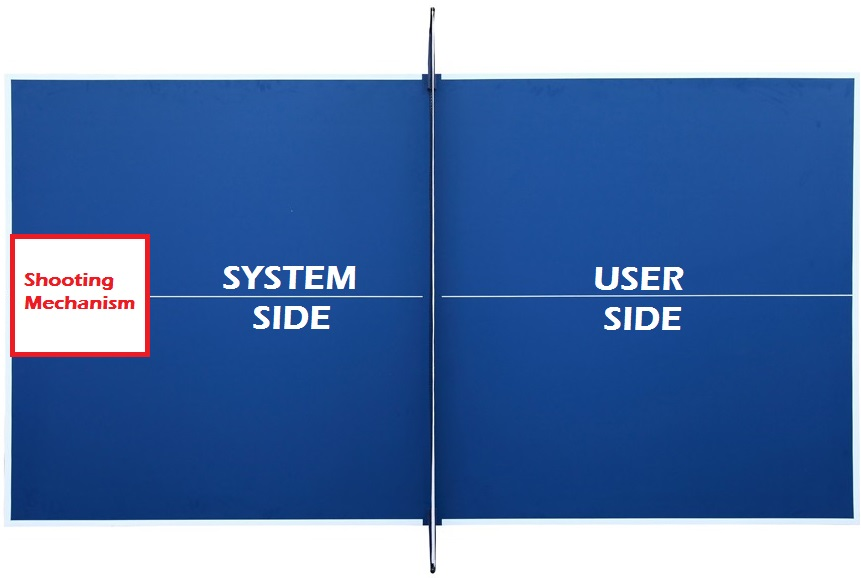
\includegraphics[width=1\textwidth]{img/table-tennis-top-view.jpeg} %requires the graphicx package
   \caption{Top View of the Tennis Table}
   \label{fig:table-tennis-top-view}
\end{figure}

\subsection{Relevant Facts \& Assumptions}
According to the International Table Tennis Federation (ITTF), the regulation table size is as follows: 2.74m long, 1.525m wide and 0.76m high off the ground. The table must be a uniformly dark colour with a 2cm-thick white line along the edge of the table, as well one running parallel to the 2.74m side in the middle of the table. The net in the middle of the table must be 15.25cm vertically high from the table. A 3D representation of the table setup is illustrate in Figure \ref{fig:table-tennis-dim}. The size of a regulated table tennis ball can be either 37mm or 40mm depending on the regulation body. For this project, the \hyperref[sec:definitions]{team} will be using 40mm balls and recommends users to do the same for optimal performance. \\
\begin{figure}[htbp]
   \centering
   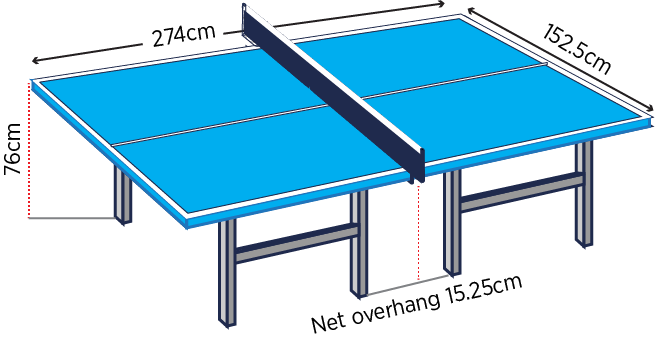
\includegraphics[width=0.7\textwidth]{img/table-tennis-dim.png} % requires the graphicx package
   \caption{3D Tennis Table with Dimensions}
   \label{fig:table-tennis-dim}
   % The Laws of Table Tennis. ITTF Handbook 2016. www.ittf.com/ittf_handbook/ittf_hb.html
\end{figure} \\
During gameplay, a valid serve must hit the \hyperref[sec:definitions]{server side} first, and then bounce once on the other player's side before being returned. After that is done, a valid return would be when the ball is hit by a player, after bouncing exactly once on their side, and bounces at least one time on the opposing player's side. If a serve touches the net and lands on the opposing player's side, it is a \textit{let}. No points are allocated and the turn must be re-served. 


\section{Project Drivers}
\subsection{Purpose}
% should include problem, lack of current solutions and ideal solution
When a player wants to improve their table tennis game, a typical solution is to hire a coach. However, this does not come without its challenges. Some of these challenges include scheduling, focusing on particular shots and receiving in-depth statistical feedback. Our proposed solution will consist of a shooting mechanism, a way to identify successful returns and a system to recommend different shots. Throughout the training session, the \hyperref[sec:definitions]{system} will provide the user with crucial feedback on the quality of their game. The system will consist of a electromechanical system to shoot the ball and a computer vision system to track the ball's location during flight. A server will also be added to store data, provide diagnostics and recommend shots given the user's past performance.
\subsection{Key Stakeholders}
\subsubsection{Client}
The client for this project comprises of the core development \hyperref[sec:definitions]{team} as both the idea and the project execution will be undertaken by the \hyperref[sec:definitions]{team}. It is also important to note that the project adviser, Dr. Alan Wassyng as well as his teaching assistants, will also be involved in the project execution in order to provide guidance and critical feedback to the project \hyperref[sec:definitions]{team}.
\subsubsection{Users}
The primary users of this project are table tennis players. Our proposed \hyperref[sec:definitions]{system} will adapt to various playing styles and levels, and hence segmenting those players down further is not required at this stage. These users are more likely to play competitively, but could also play recreationally with friends or within a club focused around the sport. \\\\
The secondary users of this project are table tennis coaches. Although this \hyperref[sec:definitions]{system} could replace a coach, a coach could find value in using this system to aid in training and assisting multiple players at one time. The system will provide analytics on players performance that can be very useful when training someone over a long period of time.
\subsubsection{Faculty}
The Department of Computing and Software is also a key stakeholder for this project. The development \hyperref[sec:definitions]{team} are students of this department and would thus represent it through the work they perform. This project is also the amalgamation of the knowledge attained by the \hyperref[sec:definitions]{team} over their undergraduate degrees. If the project is unsuccessful, the department loses the opportunity to showcase it for future students and donors.

\section{Project Scope}
\subsection{The Scope of the Work and the Product}
In order to make the project feasible within the time constraint imposed on the \hyperref[sec:definitions]{team}, it will need to be scoped accordingly. One way we are scoping the project is by limiting the types of shots the \hyperref[sec:definitions]{system} can take. A return by the system would first contact the table on the \hyperref[sec:definitions]{\textit{User side}} where a serve would first contact the table on the \hyperref[sec:definitions]{\textit{System side}}. We are limiting the system to only preform returns which excludes serves. The system will also make no attempt at returning any shots returned by the user. \\\\
After the user has returned a shot from the system, the system will not make any attempts to return a shot that is likely to be returned given the user's returns. This is to give the system the ability to focus on a particular type of shot the user is the least proficient at returning. The characteristics of the shot following any return will be determined by the system's mode and the proficiency of the player if required and available.
\subsubsection{Individual Product Use Cases}
The actors which will be interacting with the \hyperref[sec:definitions]{system} are the \textbf{trainee}, the \textbf{coach} and the \textbf{system administrator}. It is not necessary for a coach to be present, but they will have the ability to use the system alongside the trainee. See Figure \ref{fig:usecase} for the use case diagram. The following list contains all primary use cases:
\begin{itemize}
\item A trainee enters their login information
\item If the login information is correct, a trainee opens their training session on the \hyperref[sec:definitions]{system}
\item A trainee begins the training session
\item A trainee selects a training mode
\item A trainee pauses the training session
\item When the system is paused, a trainee ends the training session
\item A trainee inspects their performance
\end{itemize}
The following are secondary use cases:
\begin{itemize}
\item A coach inspects trainee's performance
\item A coach adjusts training parameters during training session
\item A system administrator calibrates the system for new tables of a non-regulation size
\end{itemize}

\begin{figure}[H]
   \centering
   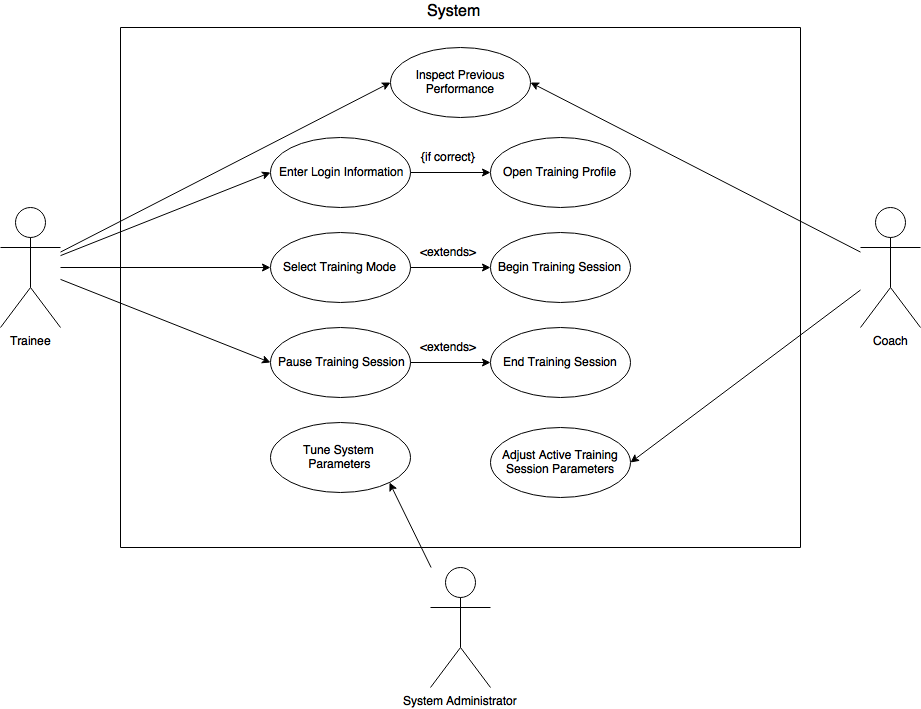
\includegraphics[width=0.7\textwidth]{diagrams/UseCase.png}
   \caption{Use Case Diagram}
   \label{fig:usecase}
\end{figure}
\subsection{Mandated Constraints}
The first constraint placed on the project is time. The deliverable and presentation dates have been set, concluding with the presentations booked for April 28, 2018. Therefore, the \hyperref[sec:definitions]{team} must successfully submit all of the deliverables and complete the project by April 28th, 2018. Additionally, a budget constraint of \$750 on the Bill of Materials (BOM) of the final product is also enforced.
\subsection{Unexpected Behaviour} 
The shooting mechanism should not start, pause or end a session without the user triggering the event. The \hyperref[sec:definitions]{system} must also refrain from shooting the ball outside the speed and angle ranges specified. Furthermore, the system should not attempt to shoot balls. \\\\
the system should attempt to shoot balls when the system runs out or something.



\subsection{Context Diagram}
\begin{figure}[H]
   \centering
   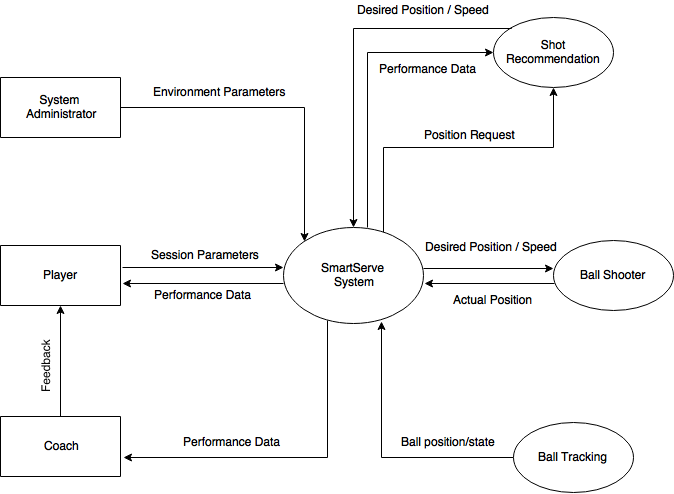
\includegraphics[width=\textwidth]{diagrams/ContextDiagram.png}
   \caption{Context Diagram}
   \label{fig:ContextDiagram}
\end{figure}


\section{Functional Decomposition Diagram}
\begin{figure}[H]
   \centering
   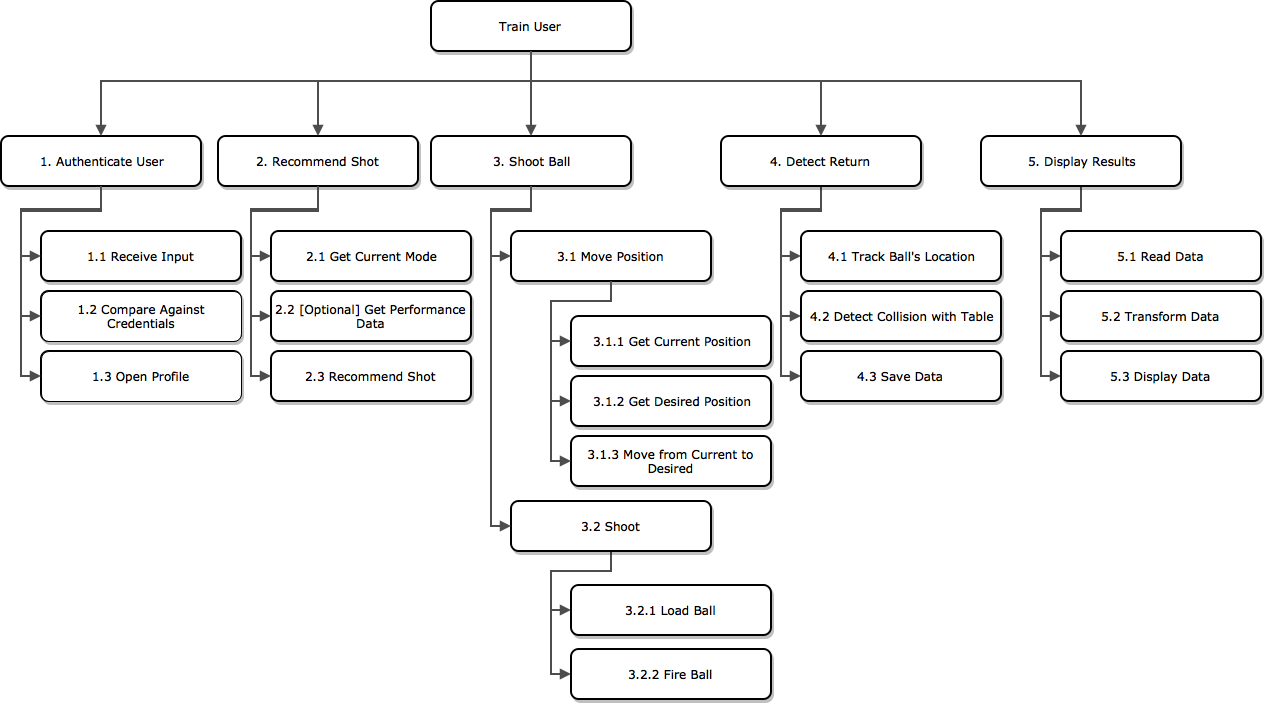
\includegraphics[width=\textwidth]{diagrams/FDD.png}
   \caption{Functional Decomposition Diagram}
   \label{fig:fdd}
\end{figure}

\section{Functional Requirements}

\begin{framed}
	\noindent\textbf{Requirement ID}: F1 \hfill \textbf{Requirement Type}: F \hfill\\\\
	\noindent\textbf{Description}: The \hyperref[sec:definitions]{shooting mechanism} shoots the table tennis ball towards the \hyperref[sec:definitions]{user side} at various locations \\
	\textbf{Rationale}: Provides variability in the shots made towards the user \\
	\textbf{Fit Criterion}: The \hyperref[sec:definitions]{shooting mechanism} can hit a specified section of a 4x4 grid with an accuracy of 75\%\\\\
	\textbf{Originator}: Sharon Platkin \\\\
	\textbf{Priority}: High \hfill \\
	\noindent\textbf{History}: Created Oct. 20, 2017
\end{framed}

\begin{framed}
	\noindent\textbf{Requirement ID}: F2 \hfill \textbf{Requirement Type}: F \hfill\\\\
	\noindent\textbf{Description}: The \hyperref[sec:definitions]{shooting mechanism} shoots the table tennis ball towards the \hyperref[sec:definitions]{user side} at various speeds \\
	\textbf{Rationale}: Provides variability in the shots made towards the user \\
	\textbf{Fit Criterion}: The \hyperref[sec:definitions]{shooting mechanism} can shoot at speeds ranging from 3 to 6 m/s at discrete increments of 0.25 \\\\
	\textbf{Originator}: Sharon Platkin \\\\
	\textbf{Priority}: High \hfill \\
	\noindent\textbf{History}: Created Oct. 20, 2017
\end{framed}

\begin{framed}
	\noindent\textbf{Requirement ID}: F3 \hfill \textbf{Requirement Type}: F \hfill\\\\
	\noindent\textbf{Description}: The \hyperref[sec:definitions]{shooting mechanism} shoots the table tennis ball towards the \hyperref[sec:definitions]{user side} at various angles \\
	\textbf{Rationale}: Provides variability in the shots made towards the user \\
	\textbf{Fit Criterion}: The \hyperref[sec:definitions]{shooting mechanism} can shoot the ball at -45 and 45 degrees relative to the longest bisection of the table at discrete increments of 1 degree\\\\
	\textbf{Originator}: Sharon Platkin \\\\
	\textbf{Priority}: High \hfill \\
	\noindent\textbf{History}: Created Oct. 20, 2017
\end{framed}

\begin{framed}
	\noindent\textbf{Requirement ID}: F4 \hfill \textbf{Requirement Type}: F \hfill\\\\
	\noindent\textbf{Description}: The \hyperref[sec:definitions]{shooting mechanism} shoots the table tennis ball towards the \hyperref[sec:definitions]{user side} at various degrees of pitch \\
	\textbf{Rationale}: Provides variability in the shots made towards the user \\
	\textbf{Fit Criterion}: The \hyperref[sec:definitions]{shooting mechanism} can shoot the ball at 0 to 55 degrees relative to the table's surface at discrete increments of 1 degree\\\\
	\textbf{Originator}: Sharon Platkin \\\\
	\textbf{Priority}: High \hfill \\
	\noindent\textbf{History}: Created Oct. 20, 2017
\end{framed}

\begin{framed}
	\noindent\textbf{Requirement ID}: F5 \hfill \textbf{Requirement Type}: F \hfill\\\\
	\noindent\textbf{Description}: The \hyperref[sec:definitions]{shooting mechanism} shoots the table tennis ball towards the \hyperref[sec:definitions]{user side} of the table with spin along 2 axes \\
	\textbf{Rationale}: Provides variability in the shots made towards the user \\
	\textbf{Fit Criterion}: The \hyperref[sec:definitions]{shooting mechanism} can spin the ball at 0 to 360 degrees in discrete increments of 45 degrees on the longitudinal axis\\\\ % longitudinal - refers to lengthwise as opposed to across
	\textbf{Originator}: Sharon Platkin \\\\
	\textbf{Priority}: High \hfill \\
	\noindent\textbf{History}: Created Oct. 20, 2017
\end{framed}

\begin{framed}
	\noindent\textbf{Requirement ID}: F6 \hfill \textbf{Requirement Type}: F \hfill\\\\
	\noindent\textbf{Description}: The \hyperref[sec:definitions]{system} can detect a successful return by the user \\
	\textbf{Rationale}: Allows quantitative information to be collected on the user's performance \\
	\textbf{Fit Criterion}: The system must detect 90\% of all successful returns made by the user\\\\
	\textbf{Originator}: Sharon Platkin \\\\
	\textbf{Priority}: High \hfill \\
	\noindent\textbf{History}: Created Oct. 20, 2017
\end{framed}

\begin{framed}
	\noindent\textbf{Requirement ID}: F7 \hfill \textbf{Requirement Type}: F \hfill\\\\
	\noindent\textbf{Description}: The \hyperref[sec:definitions]{system} saves the details for each shot taken by the shooting mechanism \\
	\textbf{Rationale}: Serves the purpose of saving the state and resuming sessions over time \\
	\textbf{Fit Criterion}: After each shot is returned, an \hyperref[sec:definitions]{ACID} (atomic, consistent, isolated and durable) transaction takes place \\\\
	\textbf{Originator}: Christopher McDonald \\\\
	\textbf{Priority}: Medium \hfill \\
	\noindent\textbf{History}: Created Oct. 20, 2017
\end{framed}

\begin{framed}
	\noindent\textbf{Requirement ID}: F8 \hfill \textbf{Requirement Type}: F \hfill\\\\
	\noindent\textbf{Description}: The \hyperref[sec:definitions]{system} can load a previously saved state \\
	\textbf{Rationale}: This will allow the user to continue a training session at different times, even if the system is powered down \\
	\textbf{Fit Criterion}: \\\\
	\textbf{Originator}: Christopher McDonald \\\\
	\textbf{Priority}: Medium \hfill \\
	\noindent\textbf{History}: Created Oct. 20, 2017
\end{framed}

\begin{framed}
	\noindent\textbf{Requirement ID}: F9 \hfill \textbf{Requirement Type}: F \hfill\\\\
	\noindent\textbf{Description}: The \hyperref[sec:definitions]{system} allows the creation of a new user \\
	\textbf{Rationale}: This allows many users to use one system \\
	\textbf{Fit Criterion}: A user must be able to be created only if the user does not already exist in the system \\\\
	\textbf{Originator}: Christopher McDonald \\\\
	\textbf{Priority}: Medium \hfill \\
	\noindent\textbf{History}: Created Oct. 20, 2017
\end{framed}

\begin{framed}
	\noindent\textbf{Requirement ID}: F10 \hfill \textbf{Requirement Type}: F \hfill\\\\
	\noindent\textbf{Description}: The \hyperref[sec:definitions]{system} must authenticate users \\
	\textbf{Rationale}: This will ensure a user can access their profile and restrict other users from accessing their profile \\
	\textbf{Fit Criterion}: No user can access another user's profile and will have access to their own 99\% of the system's uptime \\\\
	\textbf{Originator}: Christopher McDonald \\\\
	\textbf{Priority}: High \hfill \\
	\noindent\textbf{History}: Created Oct. 20, 2017
\end{framed}

\begin{framed}
	\noindent\textbf{Requirement ID}: F11 \hfill \textbf{Requirement Type}: F \hfill\\\\
	\noindent\textbf{Description}: The \hyperref[sec:definitions]{system} can pause the shooting mechanism \\
	\textbf{Rationale}: A user may need to attend other matters during training or get real-time feedback from the system \\
	\textbf{Fit Criterion}: After instantiating the pause process, the system shoots at most 1 more ball(s) \\\\
	\textbf{Originator}: Christopher McDonald \\\\
	\textbf{Priority}: High \hfill \\
	\noindent\textbf{History}: Created Oct. 20, 2017
\end{framed}

\begin{framed}
	\noindent\textbf{Requirement ID}: F12 \hfill \textbf{Requirement Type}: F \hfill\\\\
	\noindent\textbf{Description}: The \hyperref[sec:definitions]{system} can end the training session \\
	\textbf{Rationale}: This will be used when a user is done training \\
	\textbf{Fit Criterion}: \\\\
	\textbf{Originator}: Christopher McDonald \\\\
	\textbf{Priority}: High \hfill \\
	\noindent\textbf{History}: Created Oct. 20, 2017
\end{framed}

\begin{framed}
	\noindent\textbf{Requirement ID}: F13 \hfill \textbf{Requirement Type}: F \hfill\\\\
	\noindent\textbf{Description}: The \hyperref[sec:definitions]{system} can display the user's performance over a determined time range \\
	\textbf{Rationale}: This will aid the user in diagnosing their ability to play table tennis \\
	\textbf{Fit Criterion}: N/A\\\\
	\textbf{Originator}: Christopher McDonald \\\\
	\textbf{Priority}: High \hfill \\
	\noindent\textbf{History}: Created Oct. 20, 2017
\end{framed}

\begin{framed}
	\noindent\textbf{Requirement ID}: F14 \hfill \textbf{Requirement Type}: F \hfill\\\\
	\noindent\textbf{Description}: The \hyperref[sec:definitions]{system} has a \textbf{training} mode \\
	\textbf{Rationale}: This mode will focus on playing to the user's weaknesses more so than others \\
	\textbf{Fit Criterion}: After 100 pseudo-randomly distributed shots, the system will begin to distribute the shots differently. By ordering each class of shot from the least to most returned, the first 15\%, the next 35\% and the last half will all receive an equal share of shots. \\\\
	\textbf{Originator}: Christopher McDonald \\\\
	\textbf{Priority}: High \hfill \\
	\noindent\textbf{History}: Created Oct. 20, 2017
\end{framed}

\begin{framed}
	\noindent\textbf{Requirement ID}: F15 \hfill \textbf{Requirement Type}: F \hfill\\\\
	\noindent\textbf{Description}: The \hyperref[sec:definitions]{system} has a \textbf{one-shot} mode \\
	\textbf{Rationale}: This mode will focus on playing to one particular class of shot, as described by the user \\
	\textbf{Fit Criterion}: For all shots performed in this mode, 90\% must be classified as the same as the one entered \\\\
	\textbf{Originator}: Christopher McDonald \\\\
	\textbf{Priority}: Medium \hfill \\
	\noindent\textbf{History}: Created Oct. 20, 2017
\end{framed}

\begin{framed}
	\noindent\textbf{Requirement ID}: F16 \hfill \textbf{Requirement Type}: F \hfill\\\\
	\noindent\textbf{Description}: The \hyperref[sec:definitions]{system} allows a user to adjust training parameters during a session which is active or paused \\
	\textbf{Rationale}: A coach may want to push a player to train in a particular area \\
	\textbf{Fit Criterion}:  \\\\
	\textbf{Originator}: Christopher McDonald \\\\
	\textbf{Priority}: Low \hfill \\
	\noindent\textbf{History}: Created Oct. 20, 2017
\end{framed}

\begin{framed}
	\noindent\textbf{Requirement ID}: F17 \hfill \textbf{Requirement Type}: F \hfill\\\\
	\noindent\textbf{Description}: The \hyperref[sec:definitions]{system} can be calibrated for the size of the table \\
	\textbf{Rationale}: As performed by a system administrator, it should be usable for all non-regulation table sizes \\
	\textbf{Fit Criterion}: The system follows all documented requirements \\\\
	\textbf{Originator}: Christopher McDonald \\\\
	\textbf{Priority}: High \hfill \\
	\noindent\textbf{History}: Created Oct. 20, 2017
\end{framed}

\begin{framed}
	\noindent\textbf{Requirement ID}: F18 \hfill \textbf{Requirement Type}: F \hfill\\\\
	\noindent\textbf{Description}: The \hyperref[sec:definitions]{shotting mechanism} will shoot a ball once the previous has been returned to the \hyperref[sec:definitions]{system side} or 1.5 seconds after the previous shot, whichever happens first\\
	\textbf{Rationale}: This will ensure the system is reasonably fast and keeps the user engaged, as well as compensates for more experienced players. \\
	\textbf{Fit Criterion}: N/A \\\\
	\textbf{Originator}: Christopher McDonald \\\\
	\textbf{Priority}: High \hfill \\
	\noindent\textbf{History}: Created Oct. 20, 2017
\end{framed}

\section{Non-Functional Requirements}

\subsection{Look and Feel Requirements}
\begin{framed}
	\noindent\textbf{Requirement ID}: LF1 \hfill\\\\
	\noindent\textbf{Description}: The \hyperref[sec:definitions]{system} will have a minimalist design that is easy to navigate through \\
	\textbf{Rationale}: A minimalistic design will help with user discover all the options and settings of the system  \\
	\textbf{Fit Criterion}: The user must be able to navigate to any feature from the profile page in at most two steps.  \\\\
	\textbf{Originator}: Sam Hamel \\\\
	\textbf{Priority}: Medium \hfill \\
	\noindent\textbf{History}: Created Oct. 27, 2017
\end{framed}

\subsection{Usability and Humanity Requirements}
\begin{framed}
	\noindent\textbf{Requirement ID}: UH1 \hfill\\\\
	\noindent\textbf{Description}: The \hyperref[sec:definitions]{system} must be intuitive to use \\
	\textbf{Rationale}: As the system is adding onto an existing process, it should not cause strain for the user to operate \\
	\textbf{Fit Criterion}: The user must be able to create a user in less than 30 seconds. The user must be able to initiate \textit{one-shot} mode in less than 2 minutes from opening their profile.  \\\\
	\textbf{Originator}: Christopher McDonald \\\\
	\textbf{Priority}: High \hfill \\
	\noindent\textbf{History}: Created Oct. 20, 2017
\end{framed}

\begin{framed}
	\noindent\textbf{Requirement ID}: UH2 \hfill\\\\
	\noindent\textbf{Description}: The \hyperref[sec:definitions]{system} will operate using the English language \\
	\textbf{Rationale}: Development \hyperref[sec:definitions]{team} only speaks English \\
	\textbf{Fit Criterion}: All outputs generated by the system will be in English  \\\\
	\textbf{Originator}: Sharon Platkin \\\\
	\textbf{Priority}: High \hfill \\
	\noindent\textbf{History}: Created Oct. 27, 2017
\end{framed}

\subsection{Performance Requirements}

\begin{framed}
	\noindent\textbf{Requirement ID}: P1 \hfill\\\\
	\noindent\textbf{Description}: The response time of feedback for user input must be less than or equal to 100ms \\
	\textbf{Rationale}: 100ms is the approximate maximum amount of time for the user to perceive the system as reacting instantaneously. 
    \textit{Card et al. (1991), The information visualizer: An information workspace, Proc. ACH CHI'91 Conf. (New Orleans, LA, 28 April - 2 May), 181-188} Users should feel that all inputs have been registered by the system\\
	\textbf{Fit Criterion}: Any click inputs that generate feedback must do so in at most 100ms. Example: a button click must indent the button in at most 100ms from the time it was clicked.  \\\\
	\textbf{Originator}: Sam Hamel \\\\
	\textbf{Priority}: High \hfill \\
	\noindent\textbf{History}: Created Oct. 27, 2017
\end{framed}

\begin{framed}
	\noindent\textbf{Requirement ID}: P2 \hfill\\\\
	\noindent\textbf{Description}: The update time of the user's performance must match gameplay  \\
	\textbf{Rationale}: Live Performance feedback will allow users to see valuable information during their play sessions \\
	\textbf{Fit Criterion}: Any results by any return from the player must be displayed on the \hyperref[sec:definitions]{GUI} (graphical user interface) before the player returns their next shot  \\\\
	\textbf{Originator}: Sam Hamel \\\\
	\textbf{Priority}: High \hfill \\
	\noindent\textbf{History}: Created Oct. 27, 2017
\end{framed}

\begin{framed}
	\noindent\textbf{Requirement ID}: P3 \hfill\\\\
	\noindent\textbf{Description}: The shot frequency of the \hyperref[sec:definitions]{system} shall not deviate from the users set shot frequency by more than 1 ball/s  \\
	\textbf{Rationale}: If the shot frequency varies more than one second from what the user specified, they will be able to notice the difference \\
	\textbf{Originator}: Sam Hamel \\\\
	\textbf{Priority}: High \hfill \\
	\noindent\textbf{History}: Created Oct. 27, 2017
\end{framed}

\begin{framed}
	\noindent\textbf{Requirement ID}: P4 \hfill\\\\
	\noindent\textbf{Description}: The \hyperref[sec:definitions]{system} must be able to support 1000 users \\
	\textbf{Rationale}: If the system is used by a company, they will have a large amount of users using the system\\
	\textbf{Fit Criterion}: The system can store up to a thousand user profiles and their accompanying performance history data \\\\
	\textbf{Originator}: Sam Hamel \\\\
	\textbf{Priority}: Medium \hfill \\
	\noindent\textbf{History}: Created Oct. 27, 2017
\end{framed}

\begin{framed}
	\noindent\textbf{Requirement ID}: P5 \\\\
	\noindent\textbf{Description}: The \hyperref[sec:definitions]{system} will be able to support only one user playing at a time \\
	\textbf{Rationale}: The system will not be able to differentiate between player returns if they were more than one user playing at the same time \\
	\textbf{Fit Criterion}: The system will work as expected for one player playing \\\\
	\textbf{Originator}: Sam Hamel \\\\
	\textbf{Priority}: High \hfill \\
	\noindent\textbf{History}: Created Oct. 27, 2017
\end{framed}

\subsection{Operational and Environmental Requirements}
\begin{framed}
	\noindent\textbf{Requirement ID}: OE1 \hfill\\\\
	\noindent\textbf{Description}: The software for the \hyperref[sec:definitions]{system} will be able to be run on Linux, Windows and MacOS \\
	\textbf{Originator}: Sam Hamel \\\\
	\textbf{Priority}: High \hfill \\
	\noindent\textbf{History}: Created Oct. 27, 2017
\end{framed}

\begin{framed}
	\noindent\textbf{Requirement ID}: OE2 \\\\
	\noindent\textbf{Description}: The \hyperref[sec:definitions]{system} will be functional in indoor settings with bright florescent lighting in the room \\
	\textbf{Originator}: Sam Hamel \\\\
	\textbf{Priority}: High \hfill \\
	\noindent\textbf{History}: Created Oct. 27, 2017
\end{framed}

\subsection{Maintainability and Support Requirements}
\begin{framed}
	\noindent\textbf{Requirement ID}: MS1 \\\\
	\noindent\textbf{Description}: The \hyperref[sec:definitions]{system} will be able to support adding different modes to the system\\
	\textbf{Rationale}: New modes might be deemed necessary later in development, and should be easily added into the system \\
	\textbf{Fit Criterion}: The system will be able to add new shooting modes into the system so long as no changes need to be made to the hardware \\\\
	\textbf{Originator}: Sam Hamel \\\\
	\textbf{Priority}: High \hfill \\
	\noindent\textbf{History}: Created Oct. 27, 2017
\end{framed}

\begin{framed}
	\noindent\textbf{Requirement ID}: MS2 \\\\
	\noindent\textbf{Description}: The \hyperref[sec:definitions]{system} should be able to add new metrics to analyze performance\\
	\textbf{Rationale}: More efficient and appropriate methods may be found in order to analyze player performance\\
	\textbf{Fit Criterion}: The system will be able to add new performance metrics and analysis methods so long as no changes need to be made to the hardware\\\\
	\textbf{Originator}: Sam Hamel \\\\
	\textbf{Priority}: High \hfill \\
	\noindent\textbf{History}: Created Oct. 27, 2017
\end{framed}


\subsection{Security Requirements}
\begin{framed}
	\noindent\textbf{Requirement ID}: S1 \hfill\\\\
	\noindent\textbf{Description}: The \hyperref[sec:definitions]{system} must hash all passwords for user profiles \\
	\textbf{Rationale}: If the system is compromised, no person should be able to read user's passwords in plain text. \\
	\textbf{Fit Criterion}: The system uses a hashing algorithm currently supported by NIST, the National Institute of Standards and Technology.\\\\
	\textbf{Originator}: Christopher McDonald \\\\
	\textbf{Priority}: High \hfill \\
	\noindent\textbf{History}: Created Oct. 20, 2017
\end{framed}

\begin{framed}
	\noindent\textbf{Requirement ID}: S2 \hfill\\\\
	\noindent\textbf{Description}: The \hyperref[sec:definitions]{system} must encrypt all performance data for each user \\
	\textbf{Rationale}: If the system is compromised, no person should be able to exploit an opponent's weaker aspects \\
	\textbf{Fit Criterion}: The system uses an encrypting algorithm currently supported by NIST, the National Institute of Standards and Technology.\\\\
	\textbf{Originator}: Christopher McDonald \\\\
	\textbf{Priority}: Low \hfill \\
	\noindent\textbf{History}: Created Oct. 20, 2017
\end{framed}

\subsection{Political Requirements}
\begin{framed}
	\noindent\textbf{Requirement ID}: P1\\\\
	\noindent\textbf{Description}: The \hyperref[sec:definitions]{system} must allow full read access for coaches \\
	\textbf{Rationale}: If a coach purchases this system, they should be able to analyze all players information for training purposes \\
	\textbf{Fit Criterion}: \\\\
	\textbf{Originator}: Christopher McDonald \\\\
	\textbf{Priority}: Medium \hfill \\
	\noindent\textbf{History}: Created Oct. 20, 2017
\end{framed}
\subsection{Legal \& Compliance Requirements}
\begin{framed}
	\noindent\textbf{Requirement ID}: LC1 \hfill\\\\
	\noindent\textbf{Description}: The \hyperref[sec:definitions]{system} must comply and operate for all ITTF rules and regulations \\
	\textbf{Rationale}: ITTF mandates the acceptance of all table tennis equipment and the system should work with these to be used by professional players \\
	\textbf{Fit Criterion}: The system must work for any 2 tables and nets which the ITTF has accepted \\\\
	\textbf{Originator}: Christopher McDonald \\\\
	\textbf{Priority}: High \hfill \\
	\noindent\textbf{History}: Created Oct. 20, 2017
\end{framed}
\subsection{Health and Safety Requirements}
\begin{framed}
	\noindent\textbf{Requirement ID}: HS1 \hfill\\\\
	\noindent\textbf{Description}: The \hyperref[sec:definitions]{shotting mechanism} will always hit the table at least once  \\
    %TODO: HUH?
	\textbf{Rationale}: This will give the user more time and context to react to the shot \\
	\textbf{Fit Criterion}: The system imposes limits for speed and pitch of the shot \\\\
	\textbf{Originator}: Christopher McDonald \\\\
	\textbf{Priority}: High \hfill \\
	\noindent\textbf{History}: Created Oct. 20, 2017
\end{framed}

\begin{framed}
	\noindent\textbf{Requirement ID}: HS2 \hfill\\\\
	\noindent\textbf{Description}: The \hyperref[sec:definitions]{shotting mechanism} will not shoot the ball faster than 9 m/s \\
	\textbf{Rationale}: This is 75\% of one of the world's fastest shots taken in table tennis and is unlikely to be of any practical use\\
	\textbf{Fit Criterion}: The system will constrain the speed of its shooting mechanism \\\\
	\textbf{Originator}: Christopher McDonald \\\\
	\textbf{Priority}: High \hfill \\
	\noindent\textbf{History}: Created Oct. 20, 2017
\end{framed}

\begin{framed}
	\noindent\textbf{Requirement ID}: HS3 \hfill\\\\
	\noindent\textbf{Description}: The \hyperref[sec:definitions]{system} should have no exposed electronic wiring or components \\
	\textbf{Rationale}: This will protect the user from electric shocks and the system from damage \\
	\textbf{Fit Criterion}: Only by disassembling the system should wiring and components be exposed \\\\
	\textbf{Originator}: Christopher McDonald \\\\
	\textbf{Priority}: High \hfill \\
	\noindent\textbf{History}: Created Oct. 28, 2017
\end{framed}

\begin{framed}
	\noindent\textbf{Requirement ID}: HS4 \hfill\\\\
	\noindent\textbf{Description}: The \hyperref[sec:definitions]{system} will carry warnings around moving parts \\
	\textbf{Rationale}: Moving parts can expose users to risk of pinching extremities \\
	\textbf{Fit Criterion}: Warning signs are displayed at every point of risk \\\\
	\textbf{Originator}: Christopher McDonald \\\\
	\textbf{Priority}: High \hfill \\
	\noindent\textbf{History}: Created Oct. 28, 2017
\end{framed}

\begin{framed}
	\noindent\textbf{Requirement ID}: HS5 \hfill\\\\
	\noindent\textbf{Description}: The \hyperref[sec:definitions]{system} will have a button to cease all power to the system \\
	\textbf{Rationale}: In the case of dangerous operation, the system must be able to be powered off \\
	\textbf{Fit Criterion}: One button will shut down system and is labeled as such \\\\
	\textbf{Originator}: Christopher McDonald \\\\
	\textbf{Priority}: High \hfill \\
	\noindent\textbf{History}: Created Oct. 28, 2017
\end{framed}

\section{Project Issues}
\subsection{Open Issues}
Due to the nature of the project, all aspects of it must operate proficiently in order for it to be successful. For example, one potential issue would arise if no spin must be applied to the ball. This would most likely include more than one motor, all operating at the same speed. This accuracy will be difficult to achieve given the budget constraints. \\\\
Some players may be able to hit the ball much faster than the solution we build to capture successful returns. For example, if some optical sensor is used it must be fast enough to capture the ball at the point of contact, or very close to it, in order to accurately determine if it did hit the table. \\\\
Between shots of the \hyperref[sec:definitions]{system}, it must determine where the next shot will be, get into the necessary position and shoot the ball. For some cases, the shot determination could take longer than usual or the distance between initial and final state could be far. This could jeopardize the system's ability to meet requirement F18.
\subsection{Off-the-Shelf Solutions}
% TODO add OTS solution for issue #1, Jared can you do this?
For the second issue noted in the above section, a high speed camera could be used but would exceed the budget constraint placed on this project. For example, a GoPro HERO5 camera can film at 120fps but costs \$490.%[https://www.amazon.ca/GoPro-HERO5-Black-OFFICIAL-CAMERA/dp/B01KZIF4NO/ref=pd_sbs_421_1?_encoding=UTF8&psc=1&refRID=XW9MQB6DH4DYWCZSQG6N].
Additionally, a camera which can film up to 500fps costs as much as \$999.99.%http://www.allsportsystems.com/store_images/capturbundles.htm.php#640x480x500fps
These would far constrain our budget, but would solve the issue should it arise. An alternative could be mat embedded with sensors, omitting all optical sensor requirements. A mat which is roughly one-quarter the size of what we would need to cover one side of table costs \$119.99, which includes a wireless pager and any markup costs done by the manufacturer. A total estimate for our materials can be estimated to be \$150.00.\\\\
For the third issue, faster motors could be used to make the shooting mechanism move faster. However, these also must fit in the budget and will be adjusted accordingly to do so.
\subsection{New Problems}
As of \today, no new problems exist.
\subsection{Risks}
The largest and only risk to note is potentially going over budget. This is mainly with respect to the proficiency of the sensors and motors used as it is typically positively correlated with price. 
\subsection{User Documentation \& Training}
The user should be informed on the following items in order to use the system effectively:
\begin{itemize}
\item Available training modes and their purpose
\item How to read performance charts and data
\item Load table tennis balls into the correct location
\item Ensure system is positioned correctly
\end{itemize}
\section{Likely Changes}
As noted in the Project Goals document, many of the anticipated changes include enhanced accuracy of some requirements. These include the following:
\begin{itemize}
\item F1 will be changed to a 8x8 grid and then a 16x16 grid
\item Adding a \textbf{random} shooting mode
\item Adding variable heights for the shooting mechanism
\item Adding the ability to track the ball throughout its travel across the table
\end{itemize}
%\section{Appendix}
% diagrams, tables, ... etc.
\end{document}